\section{Brief Methodology Description}\label{methodology}

For developing ontologies into the scope indicated in the previous Section,  we propose Onto\textit{Smart}, a methodology  depicted in Fig.\ref{figure3-1}. This methodology is explained in details in its Wiki\footnote{https://github.com/luisenriqueramos1977/OntoSmart}, however in this Section we provide a brief description.

Onto\textit{Smart} is divided into two main horizontal sections that identify two activity groups. The former correspond to development activities and the latter to implementation activities. The inclusion of an implementation layer implies that ontologies will be developed in an application centered context; therefore these  ontologies can be evaluated by an effectiveness criterion.


Going into a first abstraction level, \textbf{Initial Activities} are those where the ontological engineer or working team roughly defines the target domain to be modeled. Meaning that the domain shall be outlined and general objectives and purpose(s) listed. \textbf{Domain Specification} activities are then a continuation of the previous activity. In this stage the ontological engineer or working team has to focus on detailed, measurable sub-objectives and specific goals.  In other words, objective should include measurable elements , which will permit us to measure our  success level. Candidate sources of knowledge have to be proposed at this stage as well.  The type and amount of documentary sources, their size and formats have to be listed; this information is later used to define development and implementation software tools.  In most ontology development methodologies, this stage commonly rests on the definition of competency questions, to which the developed or chosen ontology has to provide answers. Competency tasks that will likely require ontology (reasoning) can also be included. 

\begin{figure}
	\begin{center}
		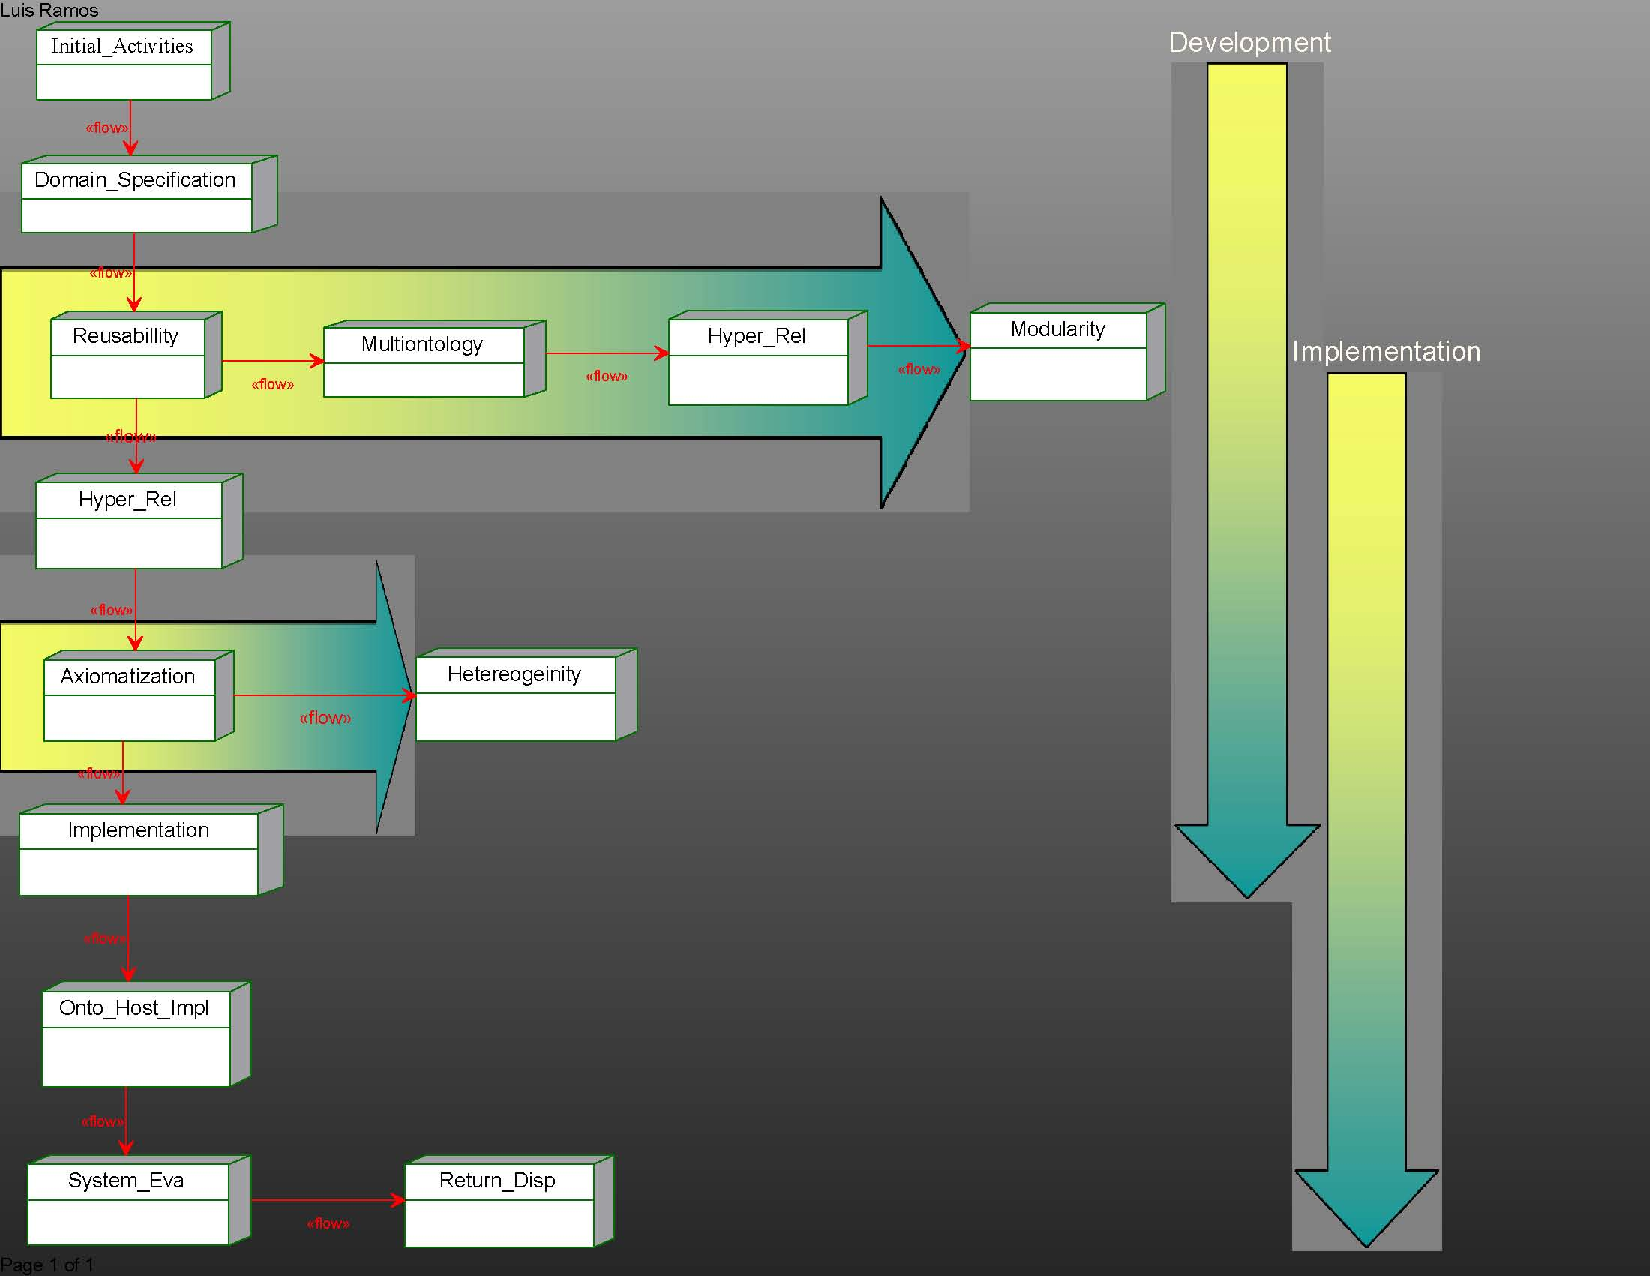
\includegraphics[scale=0.7,angle=90, totalheight = 0.8\textheight, trim=0.3cm 0.3cm 0.3cm 0.3cm, clip=true]{figure-chapterIII/figure3-22}\\
		\caption{My Methodology}
		\label{figure3-1}
	\end{center}
\end{figure}

 
We included the \textbf{Reusability}\footnote{https://github.com/luisenriqueramos1977/OntoSmart/wiki/Reusability}as a subactivity of \textbf{Modularity} because ontologies promised to be artifacts for interoperability. But to achieve this, ontologies should be managed as standardized artifacts (i.e., pieces of software). However, in most cases the use of ontologies is developed from scratch, limiting reusability and interoperability as well. In this vein, we consider worth including activities reuse and an indicator to measure reutilization level. These activities reuse consist on the following subtasks:

\begin{itemize}
	
	\item \textbf{Finding ontologies related to the target domain}\footnote{shorturl.at/gDFKZ}
	
	\item \textbf{Quality  assurance from the information point of view}\footnote{shorturl.at/bimL6}
	
	\item \textbf{First check of ontologies against requirements}\footnote{shorturl.at/dfgxT}
	
\end{itemize}


From the above described scenario we have the following possible outcomes: first, to find a fully reusable ontology is an ideal situation; second, to require development from scratch, third to develop an ontology using parts of others and fourth to reuse modular ontologies. 

To analyze the fourth scenario we require:

\begin{enumerate}
	\item Ontologies related to a common domain as input.
	\item A software tool for mapping and merging ontologies.
\end{enumerate}


Then, the current task consists in mapping all ontology against each other, so we can obtain ontological commitments amongst them.  The resulting mappings per pair of ontologies will be recorded and are maintained as a hyper-ontological structure over modules. 

At this point we should have one of the following options available: 

\begin{itemize}
	
	\item[1]. One ontology, if we have developed one from scratch, 
	\item[2].- One ontology developed from a group of ontologies, or 
	\item[3]. A set of linked (or to be linked) ontologies for reuse.  
	
\end{itemize}

After having a modular structure, we have to evaluate the necessity of \textbf{axiomatization}. That is because from the intended use of ontology, it is possible to draft the axiomatization requirements for our ontology or ontologies. In this case we need to define whether or not we need lightweight or a heavyweight ontology\footnote{https://github.com/luisenriqueramos1977/OntoSmart/wiki/Axiomatization}. As we indicated above, the existence of heavyweight ontologies indicates that the axiomatization process should be carefully considered in order to determine if the target language constructors are expressive enough to reach the expressiveness level required to fulfill our requirements. We have to be aware of the presence of n-ary relations (higher than binary), mereotopological relations, procedural reasoning and different unit systems. The  aforementioned  requirements  could possibly  enhance the expressiveness level of any language using them in a higher level. If any of them are present in the ontology or ontologies, limiting the full implementation of our model, then we should proceed with the \textbf{hetereogenity}\footnote{https://github.com/luisenriqueramos1977/OntoSmart/wiki/Heterogeneity} Building Block to determine if a heterogeneous layer is required. Otherwise, we can proceed with system implementation. In the \textbf{Implementation} Building Block, as most of Ontology methodologies, we should implement the developed ontology. However in this case, given that this methodology is centered in reutilization, it is highly likely that we should just have our ontology or ontologies developed in an ontology language. Finally, in the \textbf{System Evaluation} Building Block, we aim at assigning a quality attribute to our ontology as we currently do with any other artifact,  offering the final user a reference of the quality of the ontology as a reusable product. Here, we propose to divide our evaluation process as follows:


\begin{enumerate}
	\item[1].	 Evaluation based on the inputs, product and development process
	This evaluation is self-subdivided into the following stages:
	\begin{enumerate}
		
		\item[a.] Input quality assurance, through the input ontology evaluation procedure.
		\item[b.] Structure measurement, implementing the metrics recommended   by \cite{manouselis_exploring_2010}. These authors are of the criteria that empirical studies are needed to validate how different metrics are capable of judging deciding about quality properties and their interpretation. They developed a tool called Ontometrics, which considered metrics indicators such as Number of classes (noc), Number of Instances (noi), Number of Properties (nop), Number of Root Classes (norc), Number of leaf Classes (nolc), Averagea Population (ap), among others. 
		
		\item[c.] Modularity  , as a criterion to classify patterns, is mostly to provide judgment about quality.  Considered that implanting wrong patterns will affect the quality of the system as a whole. \cite{randelli_introducing_2010}.
		
		\item[d.] Reusability, as an average metric for reutilization, will indicate how interoperable   the system is by using inherited terms as a reference. For this task we will follow a criteria similar to the proposed by \cite{spiliopoulos_discovery_2010}, with the difference that we considered no pair, but networks of ontologies. 
		
	\end{enumerate}
	
	\item[2]. 	Evaluation related with functionally and implementation
	
	This evaluation is, in our opinion, the most crucial one, but it is subject to the system development. In other words, this evaluation will take place only when some functional part of the system is able to carry out certain tasks. For a successful evaluation, developers should have previously categorized activities, their complexity level, similar to having a list of competency questions to be answered. The criterion to define complexity will be:
	
	
	\begin{enumerate}
		
		\item[a.] If the answer to a query, or to carry out some task can  be done  through ontology, or consultation is required  for other ontologies in order to provide the required answer, or carry out the task.   
		
		\item[b.] If a decidable language is required to  execute  the corresponding tasks, but the chosen languages are not expressive enough to represent the required knowledge in the knowledgebase, such scenario will oblige us to consider a  heterogeneous framework. .  
		
	\end{enumerate}
	
\end{enumerate}


In this Section we presented a new methodology that integrates two fundamental approaches into the Ontological Engineering, those are modularity and heterogeneity. This methodology initiates with a quality assurance procedure, followed by specific method to decide when modularity and heterogeneity are required. We provides tools to support the workflow along the methodology. Furthermore,  we introduced some required technologies for implementing the proposed methodology. 

In next Section, we will present the results of implementing the just described methodology in an use case of manufacturing.